% eine Übungsaufgabe aus sabbah_cimpba90 Seite 33
% 5.3.6
% 
% zwefällt formal aber NICHT konvergent

\subsection{beispiel von sabbah}

Sei $P=t(t\partial_t)^2+t\partial_t+\frac{1}{2}$

\begin{comment}
  \begin{enumerate}
      \item zeige $\cD/\cD\cdot P$ ist ein Meromorpher Zusammenhang.
      \item Zeichne das Newton Polygon von $P$ und finde eine formale
        Aufteilung von $\cM_{\hat{K}}$.
      \item Zeige $\cM$ kann nicht in eine direkte Summe von zwei $\cD$ modulen
        zerlegt werden, dazu:
        \begin{enumerate}
          \item Zeige das die Produktzerlegung
            \[ P=(t(t\partial_t)+v(t))\cdot(t\partial_t+u(t)) \,, \]
            mit $u,v\in\Cfu$, existiert.
          \item Berechne durch Induktion die Koeffizienten von $u$.
          \item Zeige dass $u \notin \C((u))$.
        \end{enumerate}
  \end{enumerate}
\end{comment}

\subsubsection{Schritt 1} Zeige das $\cD/\cD\cdot P$ einen Meromorphen
Zusammenhag Definiert.
\subsubsection{Schritt 2}
\begin{minipage}[hbt]{0,39\textwidth}
  \begin{align*}
   P &= t(t\partial_t)^2                + t\partial_t           + \frac{1}{2}\\
     &= tt(\partial_tt)\partial_t       + t\partial_t           + \frac{1}{2}\\
     &= t^2(t\partial_t + 1)\partial_t  + t\partial_t           + \frac{1}{2}\\
     &= t^3\partial_t^2                 + (t^2 + t)\partial_t   + \frac{1}{2}\\
  \end{align*}
\end{minipage}
\begin{minipage}[hbt]{0,59\textwidth}
  \begin{center}
    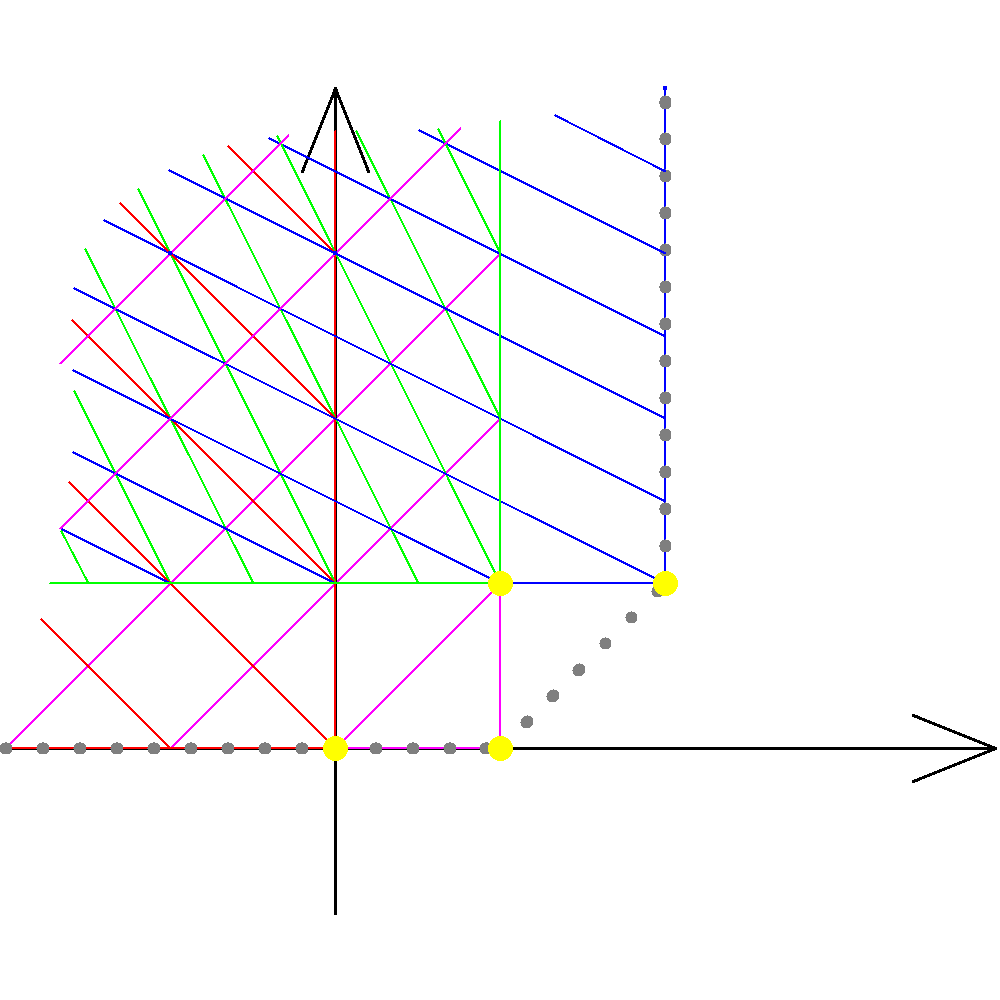
\includegraphics[width=6cm]{img/formal_a-2.png}
  \end{center}
\end{minipage}
Also mit $\slopes{P}=\{0,1\}$

\subsubsection{Schritt 3 a)}
\subsubsection{Schritt 3 b)}
\subsubsection{Schritt 3 c)}

% vim: set ft=tex :
